% mnras_template.tex
%
% LaTeX template for creating an MNRAS paper
%
% v3.0 released 14 May 2015
% (version numbers match those of mnras.cls)
%
% Copyright (C) Royal Astronomical Society 2015
% Authors:
% Keith T. Smith (Royal Astronomical Society)

% Change log
%
% v3.0 May 2015
%    Renamed to match the new package name
%    Version number matches mnras.cls
%    A few minor tweaks to wording
% v1.0 September 2013
%    Beta testing only - never publicly released
%    First version: a simple (ish) template for creating an MNRAS paper

%%%%%%%%%%%%%%%%%%%%%%%%%%%%%%%%%%%%%%%%%%%%%%%%%%
% Basic setup. Most papers should leave these options alone.
\documentclass[a4paper,fleqn,usenatbib]{mnras}

% MNRAS is set in Times font. If you don't have this installed (most LaTeX
% installations will be fine) or prefer the old Computer Modern fonts, comment
% out the following line
\usepackage{newtxtext, newtxmath}
% Depending on your LaTeX fonts installation, you might get better results with one of these:
%\usepackage{mathptmx}
%\usepackage{txfonts}

% Use vector fonts, so it zooms properly in on-screen viewing software
% Don't change these lines unless you know what you are doing
\usepackage[T1]{fontenc}
\usepackage{ae,aecompl}


%%%%% AUTHORS - PLACE YOUR OWN PACKAGES HERE %%%%%


% Only include extra packages if you really need them. Common packages are:
\usepackage{graphicx}	% Including figure files
\usepackage{amsmath}	% Advanced maths commands
\usepackage{amssymb}	% Extra maths symbols
\usepackage{mathtools}
\usepackage{url}

%%%%%%%%%%%%%%%%%%%%%%%%%%%%%%%%%%%%%%%%%%%%%%%%%%

%%%%% AUTHORS - PLACE YOUR OWN COMMANDS HERE %%%%%

% Please keep new commands to a minimum, and use \newcommand not \def to avoid
% overwriting existing commands. Example:
%\newcommand{\pcm}{\,cm$^{-2}$}	% per cm-squared
\newcommand{\dispdot}[2][.2ex]{\dot{\raisebox{0pt}[\dimexpr\height+#1][\depth]{$#2$}}}% \dispdot[<displace>]{<stuff>}

%%%%%%%%%%%%%%%%%%%%%%%%%%%%%%%%%%%%%%%%%%%%%%%%%%

%%%%%%%%%%%%%%%%%%% TITLE PAGE %%%%%%%%%%%%%%%%%%%

% Title of the paper, and the short title which is used in the headers.
% Keep the title short and informative.
\title[47 Tuc W]{On the variability of 47 Tuc W (to be decided)}

% The list of authors, and the short list which is used in the headers.
% If you need two or more lines of authors, add an extra line using \newauthor
\author[Hebbar et al.]{
Pavan R. Hebbar,$^{1}$\thanks{E-mail: hebbar@ualberta.ca}
Craig O. Heinke,$^{2}$\thanks{E-mail: heinke@ualberta.ca}
\\
% List of institutions
$^{1}$Department of Physics, University of Alberta\\
$^{2}$Department of Physics, University of Alberta\\
}

% These dates will be filled out by the publisher
\date{Accepted XXX. Received YYY; in original form ZZZ}

% Enter the current year, for the copyright statements etc.
\pubyear{2017}

% Don't change these lines
\begin{document}
\label{firstpage}
\pagerange{\pageref{firstpage}--\pageref{lastpage}}
\maketitle

% Abstract of the paper
\begin{abstract}

\end{abstract}

% Select between one and six entries from the list of approved keywords.
% Don't make up new ones.
\begin{keywords}
keyword1 -- keyword2 -- keyword3
\end{keywords}

%%%%%%%%%%%%%%%%%%%%%%%%%%%%%%%%%%%%%%%%%%%%%%%%%%

%%%%%%%%%%%%%%%%% BODY OF PAPER %%%%%%%%%%%%%%%%%%

\section{Introduction}

Neutron stars (NSs) are highly compressed objects($\rho_{center} \sim 10^{15}$g cm$^{-3}$) formed by core collapse of massive stars and supported by neutron degeneracy pressure. When the light cones from poles of highly magnetized, fast-rotating NSs sweeps across the earth, periodic radio pulses and and observed hence called radio pulsars. Millisecond pulsars
(MSPs) constitute a separate class of radio pulsars with exceptionally small periods, P $\sim 10$ ms and spin down rates, $\dispdot{P} \sim 10^{-19} - 10^{-21}$ (Lyne \& Smith 1990). From these values, it an be calculated that MSPs have magnetic fields, B $\sim 10^{17} \times (P \dispdot{P})^{1/2} = 10^{8} - 10^{9}$ G and characteristic ages, $\tau \sim P/2\dispdot{P} \sim 10^8 - 10^{10}$ yrs

Ever since the discovery of the first MSP, PSR B1937+21 (Backer et al., 1982), it has been proposed that MSPs are recycled NS that have been spun up due to accretion from a companion during their active phase.(Alpar et al. 1982, Bhattacharya \& van den Heuvel 1991). The detections of millisecond X-ray pulsations in many accreting NSs(Wijnands \& van der Klis 1998) and the observed transitions of IGR J1824-2453I(Papito et al. 2013)  and PSR J1023+0038(Archibald et al. 2009, Halpern et al. 2013, Patruno et al. 2014, Stappers et al. 2014, Tendulkar et al. 2014) between the two states  support this model for evolution of MSPs. Detailed study of PSR J1023+0038 across multiple wavelengths reveal that the low mass x-ray binary (LMXB) phase consists of three states - high flux mode ($\sim 10^{33}$ ergs s$^{-1}$) during which coherent X-ray pulsations are observed implying active accretion, low flux mode ($\sim 10^{32}$ ergs s$^{-1}$) where no pulsations have been observed probably due to accretion flow is propelled away from the pulsar and sporadic flares reaching up to $\sim 10^{34}$ ergs s$^{-1}$ (Bogdanov et al. 2015).The transition between these modes isn't associated with any spectral changes. It is observed that the X-ray emission during the radio pulsar state consists of a dominant shock component and a smaller contribution from heated magnetic polar caps that shows double-peaked pulsations. Simultaneous observations with Chandra and VLA show that the low flux modes in X-ray are associated with higher flux in radio (Bogdanov et al. 2017).

As predicted by the above model, most MSPs are found in binary systems. Binary systems with high inclinations and large stellar atmospheres show eclipses. These eclipsing binaries can be classified into two groups - black-widows with companion mass $M_2 << 0.1M_{\odot}$ and redbacks with $M_2 \sim 0.1 - 0.4M_{\odot}$. Redbacks have companions that are non degenerate low mass main sequence or subgiant stars. Recent detections of redbacks in galactic field disprove the theory that they are formed from exchange encounters. It has been proposed that the formation of redbacks differ from black widows in that the pulsar radiation is more beamed towards the companion star (Chen et al. 2013), resulting in more efficient companion evaporation rates. 

GCs are known to contain a large number of LMXBs which recycle pulsars and therefore suitable sites for searching MSPs. Since the discovery of first GC pulsar, PSR B1821-24 (Lyne et al.), more than $149$ radio pulsars have been detected in 28 GCs\footnote{For up-to-date catalog check P. Freire's website http://www.naic.edu/~pfreire/GCpsr.html} out of which $\sim$ 90\% are MSPs(Camilo \& Rasio 2005, Ransom 2007). About half of these pulsars are located in the clusters Terzan 5, 47 Tucanae and M28. About $80$ of the $138$ detected pulsars are members of binary systems. Pulsars detected in GCs are significantly different from the galactic field pulsars in that they have a greater proportion of single pulsars and short period binary pulsars, suggesting the dominant role of dynamical interactions in their formation. Also, while binary pulsars in galactic fields usually have circular orbits, $\sim$20\% of the GC binaries have highly eccentric orbits($e >$ 0.1). This can again be explained by increased dynamical interactions. Strong correlation is shown to exist between the stellar interaction rate in the cores of cluster and the number of X-ray sources in them(Pooley et al. 2003).

47 Tuc hosts 25 pulsars(all MSPs with $P\sim2-5$ms)(Camilo et al. 2000, Ridolfi et al. 2016, Freire et al. 2017) out of which 15 are binary. Radio eclipses have been detected in 5 of these pulsars of which two are confirmed to be redbacks - PSR J0024-7204W(47 Tuc W), PSR J0024-7201V(47 Tuc V). 47 Tuc W was first detected by Camilo et al.(2000) using Parkes radio telescope with a period of 2.35 ms and an orbital period of 3.2 hrs and was eclipsed for $\sim$ 25\% of its orbit. The position and the nature of the companion were deduced by matching Hubble space telescope(HST) data with the orbital period(Edmonds et al. 2002). It was found that 47 Tuc W had a main sequence companion with $M_2 > 0.13 M_{\odot}$. Detailed timing solutions have been calculated for the system which give an orbital frequency $f_b = 8.71 \times 10^{-5}$ and its derivative $\dispdot{f_b} = -1.26 \times 10^{-18}$. The position of the 47 Tuc W was coincident with that of X-ray source W29 detected by Chandra ACIS-I observation of core of 47 Tuc(Grindlay et al. 2001). X-ray analysis of 47 Tuc W showed that the emission consisted of two components - hard non thermal component that is eclipsed for $\sim$ 30\% of it's orbit which contributes to about 70\% of the observed X-ray luminosity, and a soft thermal component which did not show variability(Bogdanov et al. 2005). Bogdanov proposed that the non-thermal spectrum is from an intra-binary shock due to interaction of pulsar wind with the stellar wind and the thermal component is from the neutron star. Observations of 47 Tuc W using Chandra HRC-S in 2004-05 showed the absence of eclipses in X-ray(Cameron et al. 2007). This raises a doubt on whether 47 Tuc W is a transitional system and that it has shifted to its LMXB state. This paper uses the latest Chandra ACIS-S observations of 47 Tuc to look into this puzzle and to further investigate the system to better constrain the properties of neutron stars and the shock.

\section{Observations}

Due to the compact core of 47 Tuc, the arc-second resolution of \emph{Chandra X-ray observatory} was used to investigate the 47 Tuc W 
system. Data from ACIS-S 2002 observations(exposure of $\sim$ 300ks, PI - Grindlay, Heinke et al. 2005) and 2014-15 observations(exposure of $\sim$ 200ks, PI - Bogdanov, Bogdanov et al. 2016) have been used to 
analyze the spectrum and the X-ray light curve of the system. HRC observations of 2005-06(exposure of $\sim$ 800ks) have been also been used for the analysis of light curves.
The details of all the observations used are summarized in Table \ref{table:data}. The new observations of 2014 -- 15 have supplemented
in the detection of 50 additional sources (Bhattacharya et al., 2017) including the previously undetected X-ray
counterparts of pulsars 47 Tuc F, S, X, Z, aa with known positions.
\begin{table*}
\centering
\caption{Summary of X-ray observations used}
\label{table:data}
\begin{tabular}{cccc|ccccc}
\hline
Obs ID & Instrument & Exposure(ks) & Start Date          &  & Obs ID & Instrument & Exposure(ks) & Start Date          \\ \hline
2735   & ACIS-S     & 65.24        & 2002-09-29 16:57:56 &  & 5542   & HRC-S      & 49.76        & 2005-12-19 07:03:06 \\
3384   & ACIS-S     & 5.31         & 2002-09-30 11:37:18 &  & 5543   & HRC-S      & 50.65        & 2005-12-20 14:57:42 \\
2736   & ACIS-S     & 65.24        & 2002-09-30 13:24:28 &  & 5544   & HRC-S      & 49.83        & 2005-12-21 23:25:20 \\
3385   & ACIS-S     & 5.31         & 2002-10-01 08:12:28 &  & 5545   & HRC-S      & 51.64        & 2005-12-23 05:01:54 \\
2737   & ACIS-S     & 65.24        & 2002-10-02 18:50:07 &  & 5546   & HRC-S      & 48.27        & 2005-12-27 05:33:43 \\
3386   & ACIS-S     & 5.54         & 2002-10-03 13:37:18 &  & 6230   & HRC-S      & 44.77        & 2005-12-28 13:44:36 \\
2738   & ACIS-S     & 68.77        & 2002-10-11 01:41:55 &  & 6231   & HRC-S      & 46.89        & 2005-12-29 21:50:23 \\
3387   & ACIS-S     & 5.73         & 2002-10-11 21:22:09 &  & 6232   & HRC-S      & 44.15        & 2005-12-31 05:17:20 \\
15747  & ACIS-S     & 50.04        & 2014-09-09 19:32:57 &  & 6233   & HRC-S      & 97.18        & 2006-01-02 05:37:31 \\
15748  & ACIS-S     & 16.24        & 2014-10-02 06:17:00 &  & 6235   & HRC-S      & 49.93        & 2006-01-04 04:04:57 \\
16527  & ACIS-S     & 40.88        & 2014-09-05 04:38:37 &  & 6236   & HRC-S      & 51.7         & 2006-01-05 11:29:07 \\
16528  & ACIS-S     & 40.28        & 2015-02-02 14:23:34 &  & 6237   & HRC-S      & 49.96        & 2005-12-24 14:07:36 \\
16529  & ACIS-S     & 24.7         & 2014-09-21 07:55:51 &  & 6238   & HRC-S      & 48.2         & 2005-12-25 21:12:00 \\
17420  & ACIS-S     & 9.13         & 2014-09-30 22:56:03 &  & 6239   & HRC-S      & 49.88        & 2006-01-06 22:08:49 \\
       &            &              &                     &  & 6240   & HRC-S      & 49.07        & 2006-01-08 02:19:31 \\ \hline
\end{tabular}

\end{table*}

\subsection{Data Reduction}
CIAO version $4.9$ was used for data reduction and image processing. The initial data downloaded from WebChaSeR was reprocessed 
according to CALDB $4.7.6$ calibration standards using the \texttt{chandra\_repro} command. The parameters \texttt{`badpixel'} and \texttt{`process\_events'} were set to ``yes" in order to create new level=1 event and badpixel files using the latest calibrations. The destreak tool was run on ACIS-S4 chip to remove probable streak events by setting the parameter \texttt{`destreak'} to ``yes" during the reprocessing. In order to prevent good events from being removed, the parameter \texttt{`check\_vf\_pha'} was set to ``no". The \texttt{`pixel\_adj'} parameter was set to ``default" in order to avoid any aliasing effects from CCD pixel grids. The X-ray photons corresponding to 
$47$ Tuc W system were extracted from a circular region of $1"$ radius around the source. This region was selected as a compromise 
between selecting maximum photons from the target, and avoiding photons from the neighboring sources.
Photons were corrected for barycentric shifts using the \texttt{axbary} tool of CIAO to remove the effect of earth's motion around sun. 
The aspect solution file and the exposure statistics file were also corrected in order to correct the good time intervals. $5$ regions close to the $47$ Tuc W system free of any sources were chosen for the 
background subtraction and barycentric correction was applied on them to take the variability of background into account.

\subsection{Variability analysis}
\begin{figure}
\centering
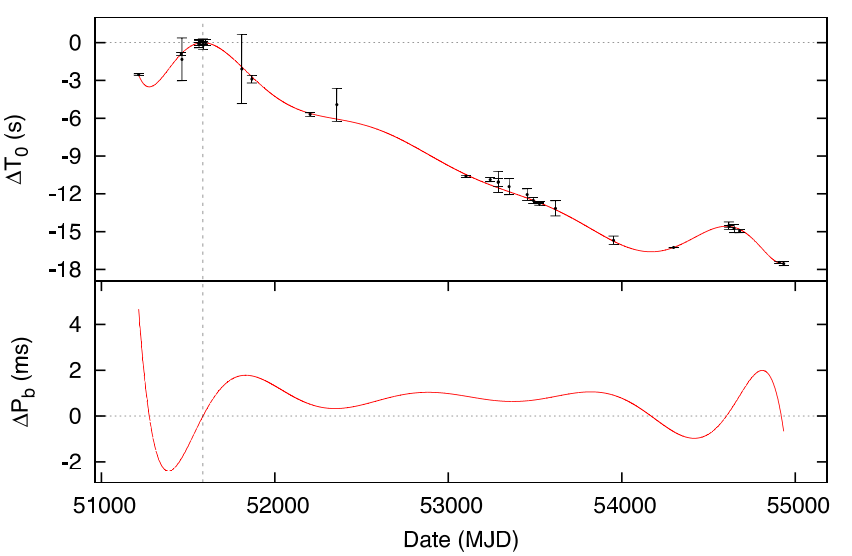
\includegraphics[width=0.5\textwidth]{Figures/ephemeris.png}
\caption{Variation in orbital parameters of 47TucW. (Top) Deviation of observed and predicted times(assuming Keplarian orbit) of passage of ascending node. (Bottom)Change in orbital period with respect to reported period in Ridolfi et al. 2016. Figure credits: Ridolfi et al. 2016}
\label{fig:ephem}
\end{figure}

The ephemeris data of 47 Tuc W system from Ridolfi et. al. 2016 (reference epoch for 47 Tuc W being MJD 50000) was used to prepare the phase folded light curve. The reported solution diverges for the 2015 data. In order to prevent this, following method was used. The graph graph of deviation of time of passage of ascending node as a function of time(Figure \ref{fig:ephem}) was approximated to a straight line. A uniform slope indicates a constant difference in the orbital frequency from it's reported value. Using this slope and the reported frequency,  the orbital frequency was calculated to be $8.70594745 \times 10^{-5}$. A
reference epoch of 51585.3327 MJD was used (time of passage of perigee). Phase folded light curves were constructed separately for
each observations from the corresponding barycenter corrected source and background files using \texttt{dmtcalc} and \texttt{dmextract}
commands. The light curves corresponding to the 2002 observations, 2004-05 observations and 2014-15 observations were added separately.
This was done to increase the number of data points and to look into any possible differences in the light curves across the three
observations. A bin size of 0.1 was used for these light curves so that the counts per bin $>10$ and gaussian error bars could be used. 
photons. In order to study the variability across different energy bands. Additional light curves were made for very low energy 
band(0.2 - 1.0 keV), low energy band(0.3 - 2.0 keV) and high energy band(2.0 - 8.0 keV) for the 2002 and 2014-15 observations 
to further study the system. For the light curves in very low energy and high energy bands, we use bin size of 0.2 to have reasonable counts in each bin.  In order to study the intra-binary shock in more detail, we also construct light curves with bin size 0.05 so that we can see the dip due to Doppler beaming more clearly.

\subsection{Spectral analysis}
The HRC observations do not contain any information regarding the energy of the photons and hence cannot be used for spectral analysis.
Data from 2002 and 2014-15 observations were analyzed separately to investigate any change in the spectrum. Too look into the nature
of the transits, the data from the intervals when the $47$ Tuc W system was in transit was grouped separately from the intervals when
the system was not in transit. For this purpose, good time intervals corresponding to the required phases, were extracted from the
\texttt{dmgti} tool and aligned to the corresponding ACIS observations using \texttt{gti\_align} tool. The spectrum from individual
observations were then extracted from \texttt{spec\_extract} tool and then combined using \texttt{combine\_spectra} in order to increase
the photon count. In order to reduce the error bars, the spectra were then grouped so that each energy bin contained a minimum number
of photons. This number was 10 for the spectrum from transit time intervals and 15 for the spectrum from remaining times. These were then analyzed in XSPEC using $\chi^2$ statistics. But this method gave large error bars on the parameters defining the model. So the spectrum were again grouped so that each bin contained a minimum of 1 photon and these were then analyzed using C-statistics. XSPEC 12.9.1 was used for the spectral analysis

\subsection{X-ray Variability}

\begin{figure}
  \centering
  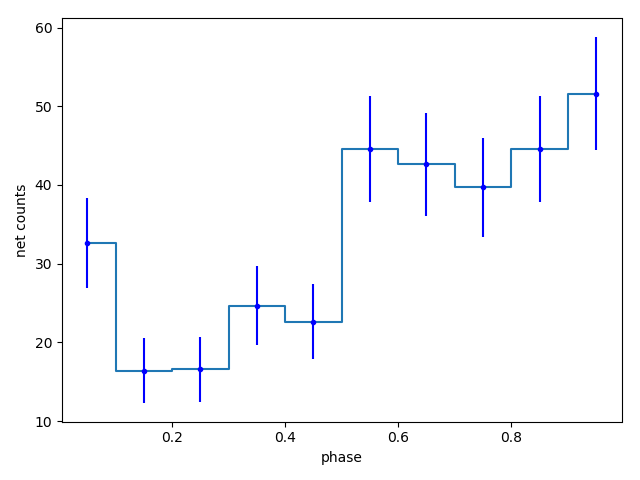
\includegraphics[width=0.5\textwidth]{Figures/2002_1filt.png}
 \caption{Phase folded light curve of 47 Tuc W from 2002 observations after background subtraction. Light curves have been folded 
 with a period of 11486.4 seconds  and a reference epoch of 51585.3327 MJD. Errors have been calculated using gehrels formulation.
 Transit can clearly be seen in the light curve from 0.1 - 0.4 phase }
 \label{fig:2002_full}
\end{figure}

\begin{figure}
 \centering
 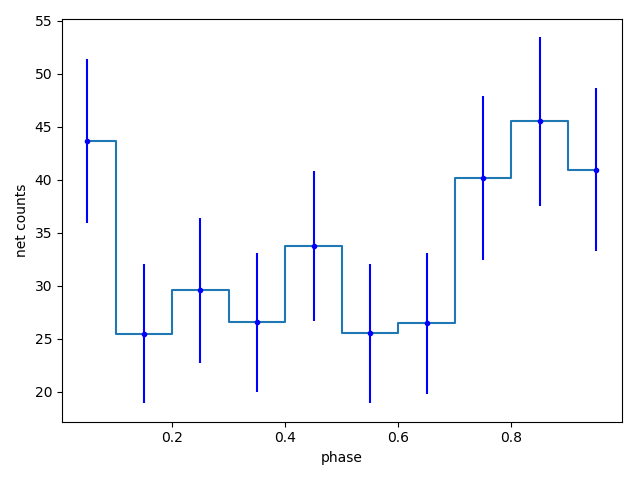
\includegraphics[width = 0.5\textwidth]{Figures/2005_1full.png}
 \caption{Phase folded light curve of 47 Tuc W from 2005 observations after background subtraction. This light curve is significantly 
 different from the one from 2002 observations. Though the light curve does show some features, they are within the error limits and 
 are not of statistical importance.}
 \label{fig:2005_full}
\end{figure}

\begin{figure}
 \centering
 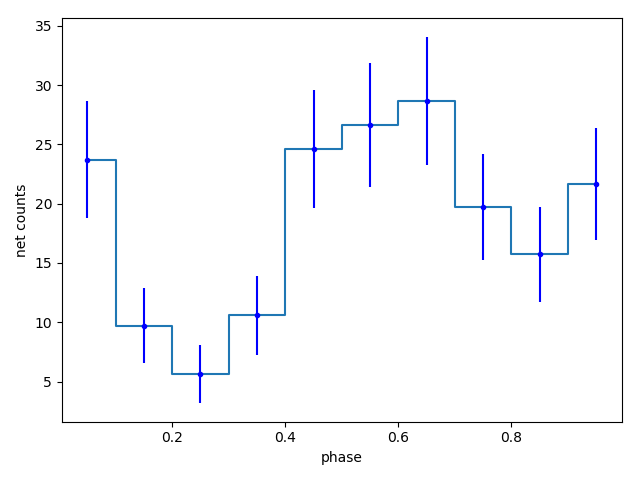
\includegraphics[width=0.5\textwidth]{Figures/2015_1filt.png}
 \caption{Phase folded light curves from 2014-15 observations. The features are very similar to the 2002 
 observations}
 \label{fig:2015_full}
\end{figure}

\begin{figure}
\centering
 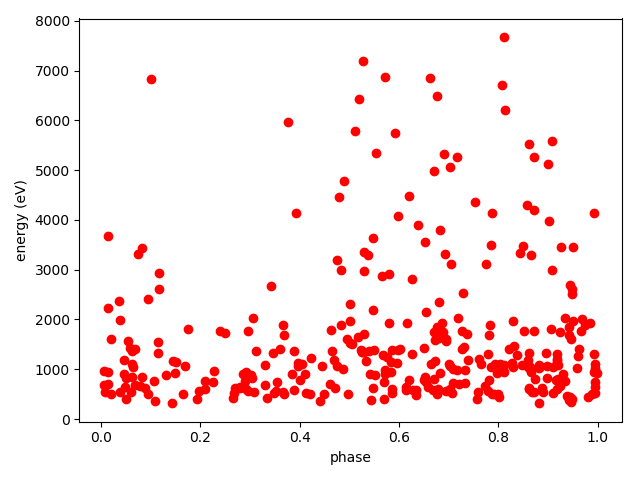
\includegraphics[width=0.5\textwidth]{Figures/2002_enph.png}
 \caption{Scatter plot of photon energy v/s phase. While the density of the points stays roughly constant in the lower energy,
 it shows significant changes for the higher energies}
 \label{fig:2002enph}
\end{figure}

\begin{figure}
 \centering
 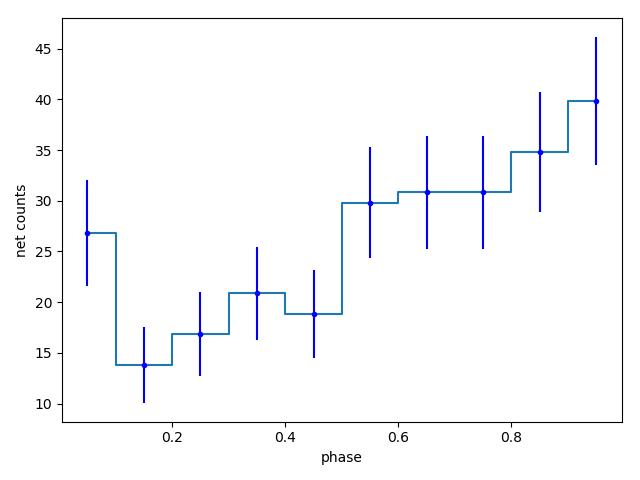
\includegraphics[width=0.5\textwidth]{Figures/2002_1low.png}  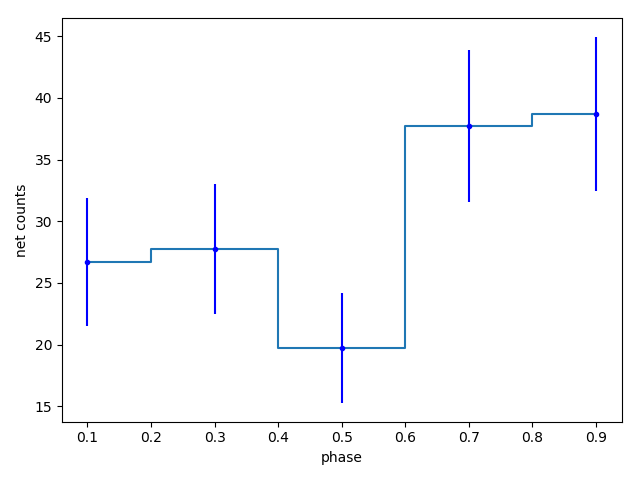
\includegraphics[width = 0.5\textwidth]{Figures/2002_1vlow.png}
 \caption{Phase folded light curves for (top)0.3 - 2.0 keV photons and (bottom)0.2 - 1.0 keV photons from ACIS 2002 observations.
 The dips in the light curve are less significant for lower energies}
 \label{fig:2002_low}
\end{figure}

\begin{figure}
 \centering
 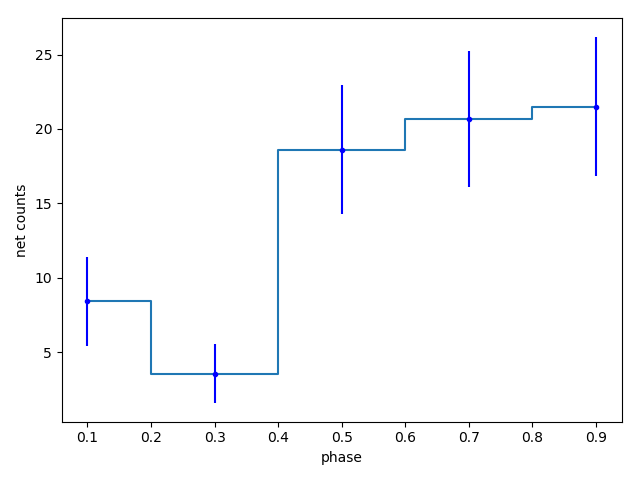
\includegraphics[width=0.5\textwidth]{Figures/2002_1high.png}
 \caption{Light curve for photons in the energy interval 2.0 - 8.0 keV. $\chi^2 = 27.2$ for a constant fit i.e probability  = $1.8 \times 10^{-5}$}
 \label{fig:2002_high}
\end{figure}

\begin{figure}
\centering
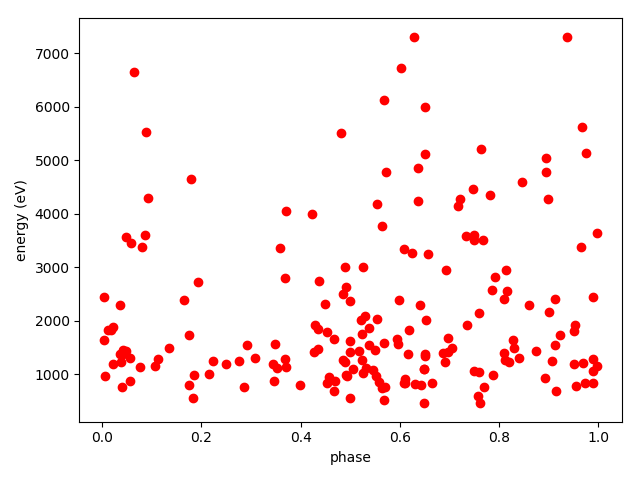
\includegraphics[width=0.5\textwidth]{Figures/2015_enph.png}
\caption{Scatter plot of energy vs phase of each photon detected. Comparing with fig. \ref{fig:2002enph}, we can see that the number of low energy photons has decreased. This is due to the reduction in the effective area of ACIS at low energies}
\label{fig:2015enph}
\end{figure}

\begin{figure}
 \centering
 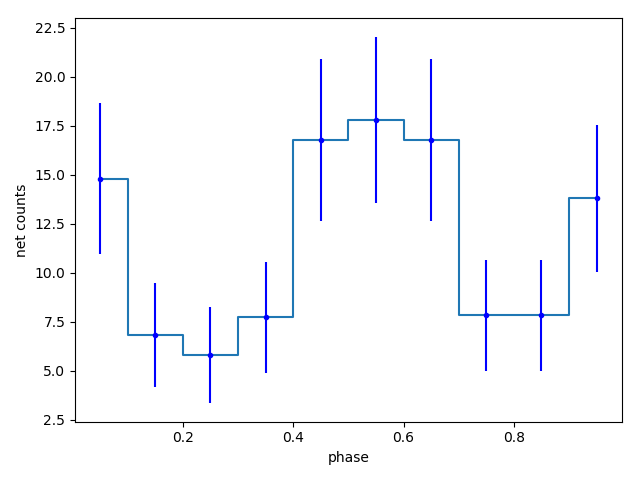
\includegraphics[width=0.5\textwidth]{Figures/2015_1low.png}
 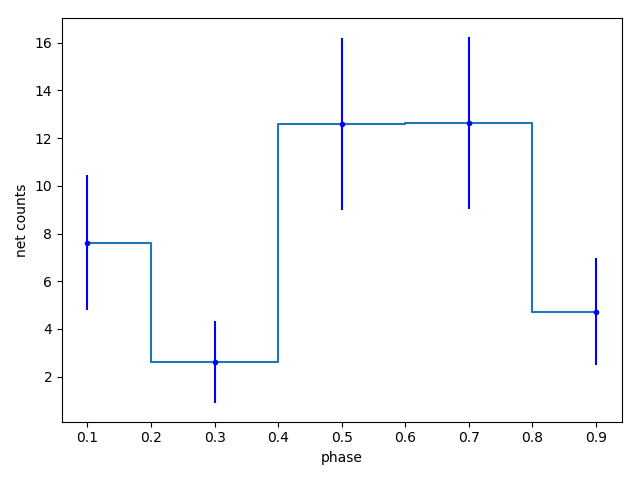
\includegraphics[width=0.5\textwidth]{Figures/2015_1vlow.png}
 \caption{Phase folded light curves for different energy bands for 2014-15 observations.(Top)Low energy photons. $\chi^2 = 17.9 \implies
 P = 0.04$ for a constant fit. (Bottom) High energy photons.
 $\chi^2 = 30.7 \implies P = 3.5 \times 10^{-6}$ for a constant fit}
 \label{fig:2015_low_high}
\end{figure}

Light curves from 2002 ACIS observations and 2004-05 HRC observation were extracted again, after accounting for the changes in the
changes in the calibration standards. Figure \ref{fig:2002_full} shows the phase folded light curve from the 2002 observations.
Dips in the light curve can be seen as pointed by Bogdonov et al. 2005. In order to confirm the nature
of these transits, the data was fit to a constant and $\chi^2$ was calculated to be $49.9$. Thus the probability of null hypothesis (no variability, $P$) is $1.1 \times 10^{-7}$, which is very small. Figure \ref{fig:2005_full} is phase folded light curve from the 2004 - 05 observations. As can
be seen from the graph the dips in the light curve are less prominent. Fitting this curve to a constant value gives
$chi^2 = 16.6$ i.e $P = 0.055$. Thus this light curve could be produced from a constant source (Cameron et al. 2007)

Figure \ref{fig:2015_full} shows the light curve extracted from the 2014 - 15 ACIS observations. Note that the light curve is very
similar to that from 2002 observations. Periodic transits in the light curve can be observed in this light curve too. The position of
these dips are slightly different due to approximations made in calculating the ephemeris of 47 Tuc W . The change in the photon count rates could be due to any intrinsic change in the source or due to the decreased effective area of Chandra in low energies. A constant fit to the light curve gives 
$\chi^2 = 42.0$  - slightly reduced because of increased errors (due to less photon counts). Thus the probability the source having a constant photon count is $3.3 \times 10^{-6}$. Thus 47 Tuc W may not have evolved much between the 2000-02 and 2014-15 observations.

To explain the difference in the 2005 light curve from the other two light curves and investigate the gross properties of the 47 Tuc W 
system, a scatter plot of photon energy v/s phase was plotted for all events as shown in figure \ref{fig:2002enph}. The density of 
points in a region depict the number of photons observed with the given energy during  a given phase. From the figure, it can be seen 
that the dips in the number of photons are much more prominent for high energy photons as compared to the lower energy photons which
shows almost no decrease. Thus the higher sensitivity of HRC detector to lower energy x-rays might be the reason for the 
absence of transits. To investigate this, light curve was plotted for  2002 observations for photons between 0.3 - 2.0 keV as shown
in figure \ref{fig:2002_low}. A constant fit to this light curve gives $\chi^2 = 26.6$ i.e probability of null hypothesis is 0.002. Since this probability is lower than that from 2005 light curve, the photons were further restricted
to energy interval 0.2 - 1.0 keV and corresponding light curve was plotted in figure \ref{fig:2002_low}. Bin size was increased to 0.2 so that each bin has reasonable number of photons. This reduces $\chi^2$ to $9.01$ i.e probability that the source has a constant light curve in this range is $0.06$ - approximately equal to that of 2005 light curve.
This could imply that the differences in the light curves of ACIS and HRC 
observations could be due to observational bias because of the difference in the sensitivity of the two detectors. On the other hand, 
in figure \ref{fig:2002_high} - the light curve for high energy photons(3.0 - 8.0 keV) from the ACIS 2002 observations, the change in 
counts per bin in the light curve is much more significant($\chi^2 = 27.2 \implies$ probability of source having constant light curve is $1.8 \times 10^{-5}$.

Figure \ref{fig:2015enph} shows the scatter plot of photon energy v/s photon phase for the 2014-15 observations. The effective area of ACIS has been decreasing in soft X-rays over the years. This is the reason for reduced number of low energy photons in fig. \ref{fig:2015enph}. Figure \ref{fig:2015_low_high} show the light curves of low energy and high energy photons for 2014-15 observations. Some amount of variability is observed even for low energy photons. This is because, due to reduced sensitivity of ACIS for soft X-rays, most of the photons in the low energy light curve have energies closer to 2.0 keV i.e they are from the intra-binary shock and thus show variability. The high energy light curves of 2000-02 and 2014-15 observations are similar except for a possible phase shift due to the approximations involved in phase calculation. Because of the low number of photons detected below 1.0 keV, no light curve was created for this energy regime. 

\section{X-Ray Spectrum}
\begin{figure}
 \centering
 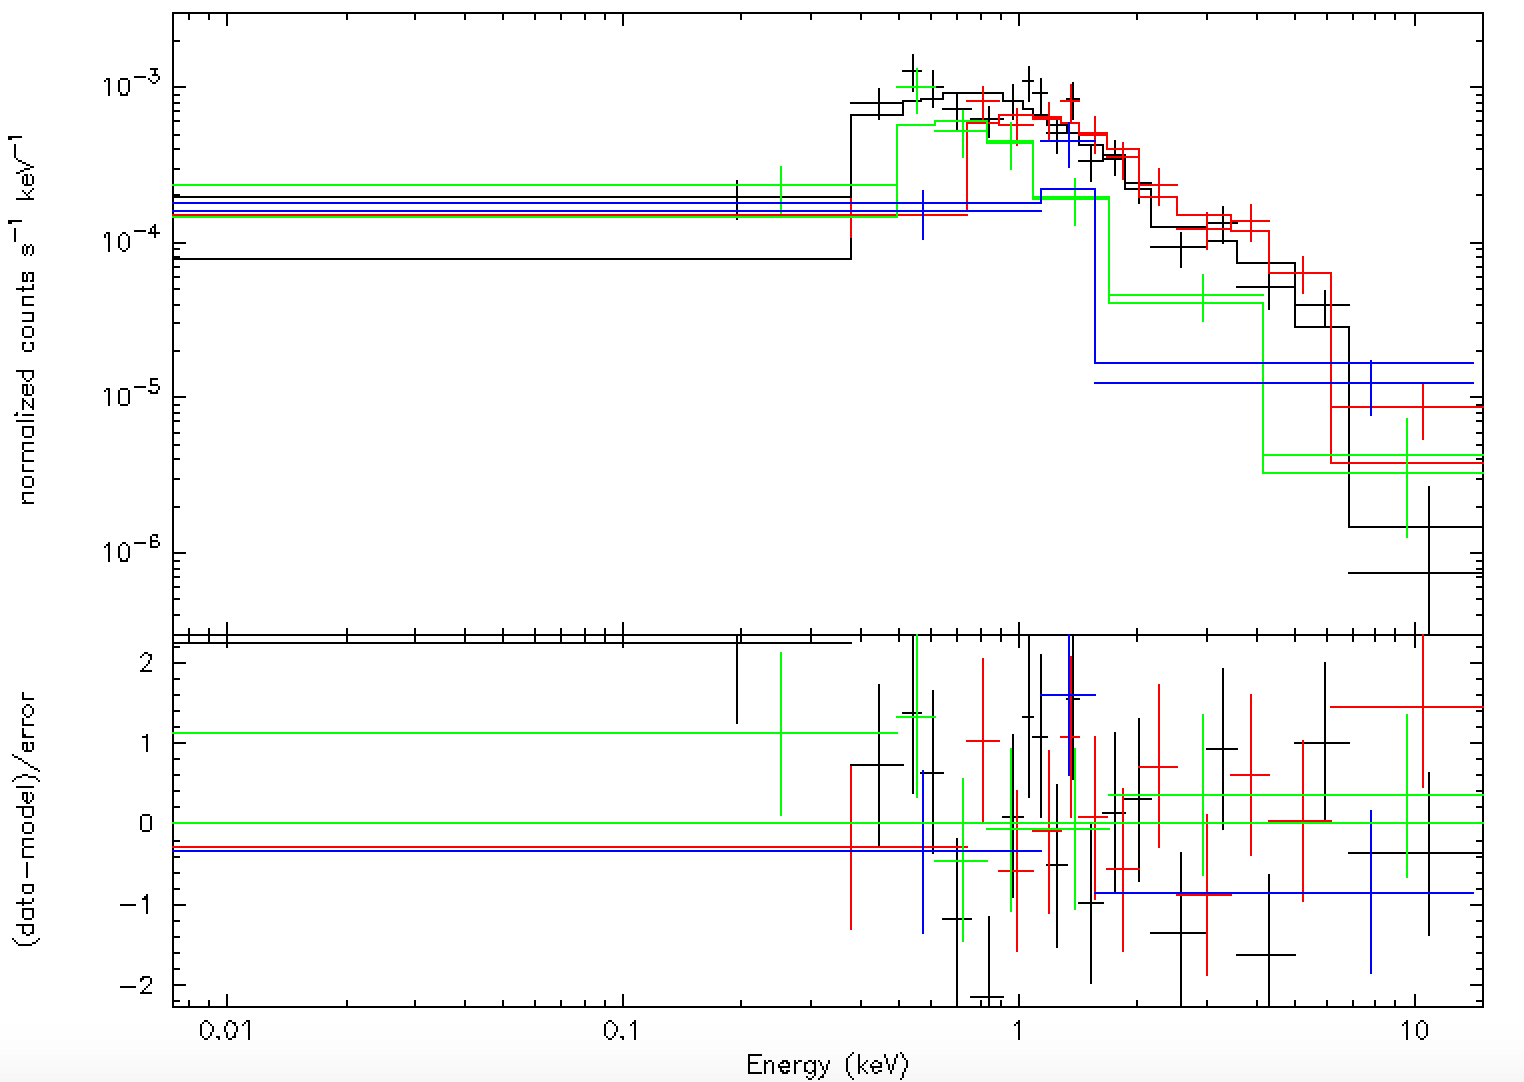
\includegraphics[width=0.5\textwidth]{Figures/blackbody.png}
 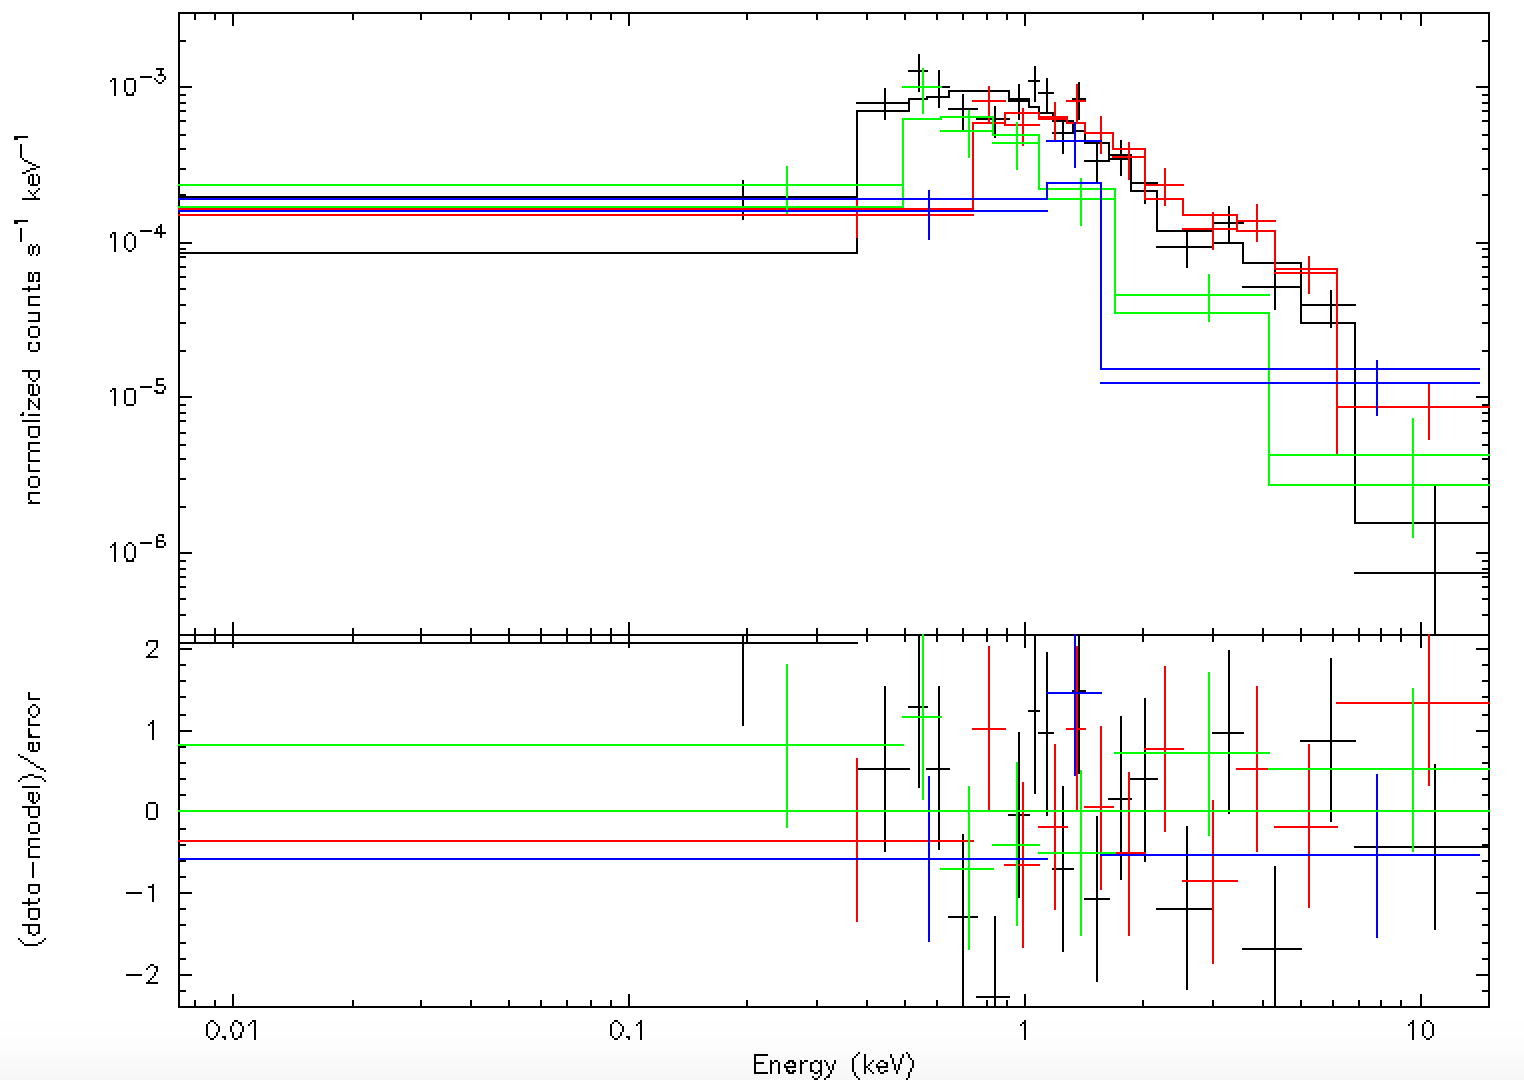
\includegraphics[width=0.5\textwidth]{Figures/nsat.png}
 \caption{Spectral fits to the observed spectrum.(Top)Model with pegged power law and blackbody components with absorption modeled
 from \texttt{tbabs}.(Bottom)Model with pegged power law and neutron star atmosphere components and absorption modeled from \texttt{tbabs}. Black refers
 to D1, red refers to D2, green refers to D3 and blue represents D4. The dotted lines represent the corresponding additive components. Though the data were fit using 1 photon groups and C-statistic, for the sake of better visualization, groups of 15 photons have been shown.}
 \label{fig:spec_fit}
\end{figure}

The X-ray spectrum for 47 Tuc W system was analyzed for 0.3 - 8.0 keV photons where ACIS instrument has highest sensitivity. Data was
divided into 4 groups to look into any changes in the spectra during eclipse and between the 2002 and 2014-15 observations:
\begin{itemize}
 \item \textbf{D1} - Data from 2002 observations extracted from phases where there is no eclipse (phases 0.0-0.1 and 0.4- 1.0)
 \item \textbf{D2} - Data from 2014-15 observations extracted from phases where there is no eclipse (phases 0.0-0.1 and 0.4-1.0)
 \item \textbf{D3} - Data from 2002 observations during the eclipse (phases 0.1-0.4)
 \item \textbf{D4} - Data from 2002 observations during the eclipse (phases 0.1-0.4)
\end{itemize}

Due to the low photon counts, data were grouped to have minimum of 1 photon per bin, and C-statistic was used to fit the models.
The hydrogen column density towards 47 Tuc was taken to be $3.5 \times
10^{20} cm^{-2}$ (Bogdanov et al. 2016) and \texttt{wilms} abundances(Wilms et al. 2000) were used. The absorptions due to dust was modeled by \texttt{tbabs} tool in XSPEC.
Due to less data points several approximations had to be made. These models and the reasoning
behind these approximations have been described below.

On plotting the data, a power law trend was observed. So all the four data groups were independently fit with a pegged power law with
0.3 keV and 8.0 keV as the energy cutoffs.(model 1). Due to the low photon count the parameters of the spectral fit of D3 and D4
had huge errors. It was observed that the photon indices of D1 and D2 were similar within 90\% confidence error bars, and same could be 
observed for D3 and D4. So the photon indices of (D1, D2) and (D3, D4) were linked to be same. Fitting a pegged power law, with linked
photon indices (model 2) gave $\Gamma = 1.49 \pm 0.12$ for D1 and D2 and $\Gamma = 2.31 \pm 0.32$. 

The large change in the value of photon index during the eclipse suggests the possibility of two sources in 47 Tuc W. The hard spectrum could be emitted from the intra-binary shock which is closer to the companion star and hence gets eclipsed for longer period of time. The softer spectrum could be thermal emission from the NS.

The soft spectrum from NS could be explained by a Blackbody (BB) (model 3) or a neutron star atmosphere model(model 4). From the parameters 
of the binary orbit of (47 Tuc W) system, it can be calculated the the neutron star is expected to be occulted for 2-5\% of the orbit.
Since the bins, where the light curve dips correspond to a larger time interval($\approx 30\%$ of the orbit), the emission from the neutron star can be assumed constant.
Thus the parameters of the softer spectrum are assumed to be same across all the data groups. 

The blackbody model was fit using the \texttt{bbodyrad} model in XSPEC. Because of the low contribution of the neutron star to the total flux, more constraints were needed to get reasonable values and error bars. Since the black body model is supposed to explain the emission in soft X-rays, the temperature was capped to a maximum of 0.3 keV. With these approximations, a good fit could be obtained for the observed spectrum with reasonable error bars.

The neutron star atmosphere model was fit using the \texttt{nsatmos} model of XSPEC. The neutron star mass was assumed to be 1.4 
solar masses and the distance to 47 Tuc W was fixed to 4.53 kpc (Bogdanov et al. 2016). Since even with these approximations the error in the parameters were
large, radius of neutron star was constrained to 10 km. Since \texttt{norm} is the fractional part of the neutron star emitting, effective radius of the emitting region was calculated. With these approximations the model could be fit with 
reasonable errors (model 4). Since \texttt{nsatmos} is a better model to explain emission from neutron star, we shall use this model for further analysis

All data have been summarized in Table \ref{table:spec_analys}. A plot of the the various elements of model 3 along with the data
is shown in figure \ref{fig:spec_fit}. Figure \ref{fig:spec_fit} also shows the various components of models 4. 

\begin{table*}
\centering
\begin{tabular}{cccccc}
\hline
Data Groups         & Model parameters & \texttt{tbabs*pegpw}                                          & \texttt{tbabs*pegpw}(linked indices)                                           & \texttt{tbabs*(pegpw+bbodyad)}                                           & \texttt{tbabs*(pegpw+nsatmos)}                                           \\ \hline
D1 & Power law index  & $1.60 \pm 0.15$                                    & $1.50 \pm 0.12$                                     & $1.16_{-0.26}^{+0.24}$                                    & $1.04_{-0.27}^{+0.26} $              \vspace{0.5em}                      \\ 
                    & Power law flux   & $1.07_{-0.13}^{+0.14} \times 10^{-14}$  & $1.13_{-0.13}^{+0.14} \times 10^{-14}$  & $1.04_{-0.15}^{+0.16} \times 10^{-14}$  & $1.01_{-0.16}^{0.17} \times 10^{-14}$ \vspace{0.5em}   \\
                    & Teff             & -                                                 & -                                                 & $1.84_{-0.58}^{+0.48} \times 10^{6}$        & $1.05_{-0.37}^{+0.36} \times 10^{6}$    \vspace{0.5em}   \\
                    & Radius          & -                                                 & -                                                 & $2.38_{-0.87}^{+2.73} \times 10^{-1}$    & $1.29_{-0.49}^{+1.61}$                                 \vspace{0.5em}        \\
                    & Thermal Flux & - & - & $1.58_{-0.61}^{+0.60} \times 10^{-15}$ & $2.02_{-0.66}^{+0.62}$  \vspace{0.5em} \\
D2 & Power law index  & $1.29 \pm 0.21$                                     & $1.50 \pm 0.12$                                     & $1.16_{-0.26}^{+0.24} $                                    & $1.04_{-0.27}^{+0.26} $                     \vspace{0.5em}                 \\
                    & Power law flux   & $1.54_{-0.22}^{+0.26} \times 10^{-14}$  & $1.42_{-0.18}^{+0.20} \times 10^{-14}$ & $1.45_{-0.21}^{+0.24} \times 10^{-14}$  & $1.45_{-0.22}^{+0.26} \times 10^{-14}$  \vspace{0.5em}  \\
                    & Teff             & -                                                 & -                                                 & $1.84_{-0.58}^{+0.48} \times 10^{6}$        & $1.05_{-0.37}^{+0.36} \times 10^{6}$   \vspace{0.5em}   \\
                    & Radius          & -                                                 & -                                                 & $2.38_{-0.87}^{+2.73} \times 10^{-1}$    & $1.29_{-0.49}^{+1.61}$                          \vspace{0.5em}           \\
                     & Thermal Flux & - & - & $1.58_{-0.61}^{+0.60} \times 10^{-15}$ & $2.02_{-0.66}^{+0.62}$  \vspace{0.5em} \\
D3 & Power law index  & $2.43_{-0.38}^{+0.40}$                                     & $2.30_{-0.31}^{+0.33}$                                     & $1.16_{-0.26}^{+0.24}$                                    & $1.04_{-0.27}^{+0.26} $        \vspace{0.5em}                              \\
                    & Power law flux   & $3.98_{-0.82}^{+0.98} \times 10^{-15}$ & $4.07_{-0.85}^{1.01} \times 10^{-15}$ & $3.04_{-1.38}^{+1.64} \times 10^{-15}$  & $2.41_{-1.29}^{+1.65} \times 10^{-15}$ \vspace{0.5em}   \\
                    & Teff             & -                                                 & -                                                 & $1.84_{-0.58}^{+0.48} \times 10^{6}$        & $1.05_{-0.37}^{+0.36} \times 10^{6}$    \vspace{0.5em}   \\
                    & Radius          & -                                                 & -                                                 & $2.38_{-0.87}^{+2.73} \times 10^{-1}$    & $1.29_{-0.49}^{+1.61}$                 \vspace{0.5em}                  \\
                     & Thermal Flux & - & - & $1.58_{-0.61}^{+0.60} \times 10^{-15}$ & $2.02_{-0.66}^{+0.62}$  \vspace{0.5em} \\
D4 & Power law index  & $2.01_{-0.56}^{+0.58}$                                       & $2.30_{-0.31}^{+0.33}$                                     & $1.16_{-0.26}^{+0.24}$                                    & $1.04_{-0.27}^{+0.26} $                \vspace{0.5em}                     \\
                    & Power law flux  & $5.03_{-1.47}^{+1.88} \times 10^{-15}$                  & $5.00_{-1.47}^{1.81} \times 10^{-15}$   & $4.38_{-2.05}^{+2.45} \times 10^{-15}$ & $3.73_{-1.92}^{2.48} \times 10^{-15}$ \vspace{0.5em}  \\
                    & Teff             & -                                                 & -                                                 & $1.84_{-0.58}^{+0.48} \times 10^{6}$        & $1.05_{-0.37}^{+0.36} \times 10^{6}$    \vspace{0.5em}   \\
                    & Radius          & -                                                 & -                                                 & $2.38_{-0.87}^{+2.73} \times 10^{-1}$    & $1.29_{-0.49}^{+1.61}$         \vspace{0.5em}       \\   
                     & Thermal Flux & - & - & $1.58_{-0.61}^{+0.60} \times 10^{-15}$ & $2.02_{-0.66}^{+0.62}$  \vspace{0.5em} \\ \hline   
\end{tabular}
\caption{Parameters of spectral fits in various models for different data groups. Power law flux is expressed in the units of ergs/cm$^2$/s, Teff in K and radius in km. D1 - Photons from 2002 observations when light curve doesn't dip, D2 - Photons from 2014-15 observations light curve doesn't dip. D3 - Photons from 2002 observations during eclipse, D4 - Photons from 2014-15 observations during eclipse. Radius refers to the radius of the region emitting non thermal radiation. Flux has been calculated between 0.3-8.0 keV. Error-bars represent 90\% confidence interval i.e $2.706\sigma$}
\label{table:spec_analys}
\end{table*}

From the values of thermal flux in Table \ref{table:spec_analys}, we see that the thermal emission is much smaller($\approx 1/5$) than the non thermal one. The radius of the region emitting thermal radiation is much smaller than the NS radius indicating the presence of hot-spots on the NS. Fixing the \texttt{norm} to 1 and varying the radius of the NS gives extremely small radius ($\sim$ 5 km), which is not possible thus proving that only a small part of the NS is radiating in soft X-rays. With a distance of 4.53 kpc, the non thermal and the luminosity can be calculated to $L_{X, NT} = 2.48_{-0.38}^{+0.42} \times 10^{31}$ ergs/s 
and $L_{X, NS} = 4.96_{-1.62}^{1.52} \times 10^{30}$ ergs/s between 0.3 - 6.0 keV for the 2002 data. The non thermal flux seems to have increased during the 2014-15 observations by $\gtrsim 5\sigma$. This could be caused because of changes in the properties of intra-binary shock. Since the pulsar doesn't evolve in such small time scales, there is probably some change in the wind from the companion star over the years.

\section{Properties of the Intra-Binary Shock (IBS) (to be discussed)}
The non thermal emission is most probably synchrotron emission(Bogdonov et al. 2005) from particles accelerated by the intra-binary shock formed due to interaction of pulsar wind and stellar wind from the main-sequence companion. Given, $\Gamma = 1.01_{-0.16}^{+0.17}$, the energy distribution of particles must be $dn/dp \propto p^{-s}$, $s = 2\Gamma + 1 = 3.08_{-0.54}^{+0.52}$, where n is the number density of particles per unit momentum and p is the magnitude of momentum. Thus, $d^3 n/dp^3 \propto p^{-\alpha}$, $\alpha = 5.08_{-0.54}^{+0.52}$. Since the pulsar wind is relativistic, we have post shock bulk modulus
$\beta_2 = (1 - \chi^2)^{-1/2}/sin\delta_1$ (Komissarov \& Lyutkov 2011), where $\delta_1$ is the angle between the bulk velocity and the shock upstream and
\begin{equation}
\chi(\sigma) = [1 + 2\sigma + (16\sigma^2 + 16\sigma + 1)^{1/2}]/(6 + 6\sigma)
\end{equation}
$\sigma$ is the ratio of magnetic and particle energy flux in the pulsar wind. 

\section{Conclusions}

With the help of additional data from 2014-15 observations, the significance of the dips in the light curve can be proved. Though the light curves of 2002 and 2014-15 data show similar features, the overall flux seems to have increased in the latter observations. With more observations and higher photon count, we could fit better spectra and check for other possible differences in the two observations.



%%%%%%%%%%%%%%%%%%%%%%%%%%%%%%%%%%%%%%%%%%%%%%%%%%

%%%%%%%%%%%%%%%%%%%% REFERENCES %%%%%%%%%%%%%%%%%%

% The best way to enter references is to use BibTeX:

%\bibliographystyle{mnras}
%\bibliography{example} % if your bibtex file is called example.bib


% Alternatively you could enter them by hand, like this:
% This method is tedious and prone to error if you have lots of references


%%%%%%%%%%%%%%%%%%%%%%%%%%%%%%%%%%%%%%%%%%%%%%%%%%

%%%%%%%%%%%%%%%%% APPENDICES %%%%%%%%%%%%%%%%%%%%%



%%%%%%%%%%%%%%%%%%%%%%%%%%%%%%%%%%%%%%%%%%%%%%%%%%


% Don't change these lines
\bsp	% typesetting comment
\label{lastpage}
\end{document}

% End of mnras_template.tex
